\documentclass[11pt]{article}
\addtolength{\oddsidemargin}{-1.cm}
\addtolength{\textwidth}{2cm}
\addtolength{\topmargin}{-2cm}
\addtolength{\textheight}{3.5cm}
\newcommand\tab[1][1cm]{\hspace*{#1}}
\usepackage[pdftex]{graphicx}
\usepackage{pdflscape}
\usepackage{tabularx}
\usepackage[T1]{fontenc}
\usepackage{hyperref}
\usepackage{float}
\usepackage{cite}
\hypersetup{
	colorlinks=true,
	linkcolor=black,
	filecolor=magenta,
	urlcolor=cyan,
}

% define the title
\author{Panda Inc}
\title{RetroRabbit - AI Game Playing Agent}
\begin{document}
\begin{titlepage}
	
	\begin{center}
		% Upper part of the page         
        
\includegraphics[width=5cm, height=5cm]{Images/PandaInc_logo.jpg}\\[0cm] 
		\textsc{\LARGE Panda Inc}\\[0.3cm]
		% Title
		\rule{\linewidth}{0.5mm} \\[1cm]
		{ \huge \bfseries RetroRabbit - AI Game Playing Agent}\\[0.5cm]
		\rule{\linewidth}{0.5mm} \\[1cm] 		
  
		
		\begin{minipage}{0.4\textwidth}
			\begin{flushleft} \large
				\emph{} \\
				Quinton {Swanepoel}
			\end{flushleft}
		\end{minipage}
		\begin{minipage}{0.4\textwidth}
			\begin{flushright} \large
				\emph{} \\
				15245510
			\end{flushright}
		\end{minipage}

		\begin{minipage}{0.4\textwidth}
			\begin{flushleft} \large
            	\emph{} \\
				Azhar {Patel}
			\end{flushleft}
		\end{minipage}
		\begin{minipage}{0.4\textwidth}
			\begin{flushright} \large
				\emph{} \\
				15052592
			\end{flushright}
		\end{minipage}
		
		\begin{minipage}{0.4\textwidth}
			\begin{flushleft} \large
				\emph{} \\
				Tshepo Macebo {Malesela}
			\end{flushleft}
		\end{minipage}
		\begin{minipage}{0.4\textwidth}
			\begin{flushright} \large
				\emph{} \\
				14211582
			\end{flushright}
		\end{minipage}

		\begin{minipage}{0.4\textwidth}
			\begin{flushleft} \large
				\emph{} \\
				Monkeli Fred {Dilapisho}
			\end{flushleft}
		\end{minipage}
		\begin{minipage}{0.4\textwidth}
			\begin{flushright} \large
				\emph{} \\
				15074260
			\end{flushright}
		\end{minipage}
        
        \begin{minipage}{0.4\textwidth}
			\begin{flushleft} \large
				\emph{} \\
				Keaton {Pennels}
			\end{flushleft}
		\end{minipage}
		\begin{minipage}{0.4\textwidth}
			\begin{flushright} \large
				\emph{} \\
				14373018
			\end{flushright}
		\end{minipage}
		
		\rule{\linewidth}{0.5mm} \\[1cm] 
		\textsc{\Large Stakeholders}\\[0cm]	
		
		\begin{minipage}{0.4\textwidth}
			\begin{flushleft} \large
				\emph{} \\
				Retro Rabbit:
			\end{flushleft}
		\end{minipage}
		\begin{minipage}{0.4\textwidth}
			\begin{flushright} \large
				\emph{} \\
				Frikkie Snyman
			\end{flushright}
		\end{minipage}

		
	\end{center}
    \tableofcontents
\end{titlepage}


\newpage

\section{Panda Inc.}
\subsection{About Us}
Panda Inc. is a team of hard working passionate software developers. Each member of the team brings their own unique, diverse skill set to the table, which includes competence in a wide range of fields such as Artificial Intelligence, multimedia and also business intellect. Panda Inc. has a fun and modern culture that promotes blue sky thinking and solutions that fit into the modern environment. The team works exceptionally well together and all members aim to produce a quality product while also creating a constructive relationship with our client.

\subsection{The Team}
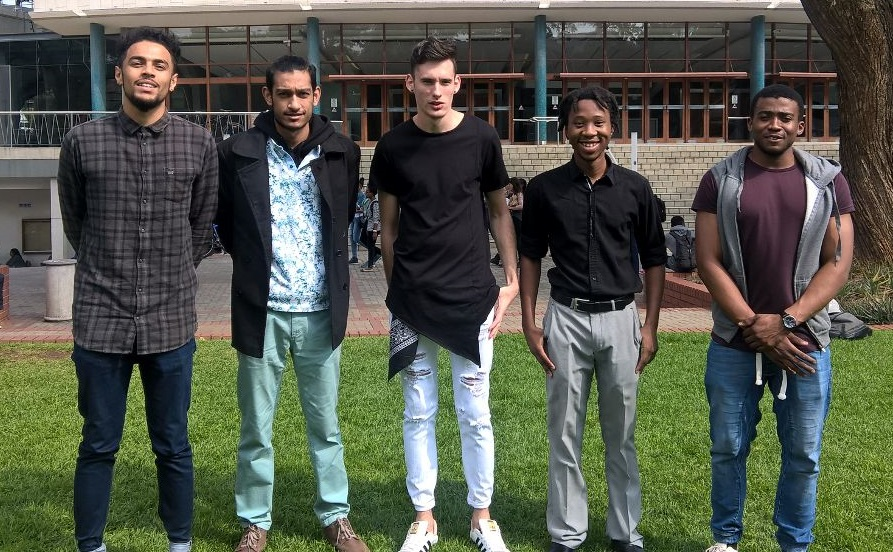
\includegraphics[width=\textwidth]{Images/Team_Pic.jpg}

\paragraph{} \textbf{Quinton Swanepoel} 
\paragraph{}Course : BSc Computer Science (with Informatics)
\paragraph{}Career Interest : Software Development / Business Systems Development  
\paragraph{}Skills : 
\begin{tabularx}{\textwidth}{
    @{\hspace{1.5em}}% Space for left bullet
    >{\leavevmode\llap{\textbullet~}\raggedright}% Left bullet + formatting of column
    X% Left column specification
    @{\quad\hspace{1.5em}}% Space between columns + right bullet space
    >{\leavevmode\llap{\textbullet~}\raggedright\arraybackslash}% Right bullet + formatting of column
    X% Right column specification
    @{}% No column space on right
  }
  Programming (C++, Java, C\#) & 
    Web Development \\
  Systems Design & 
    Mobile Development (Android Studio, Xamarin)
\end{tabularx}

\paragraph{Bio :}I started at the University of Pretoria in 2015 studying computer science, second year I  decided to start taking the prescribed BCom Informatics modules in addition to my computer science modules. This is because I love the business aspect of IT but I'm also interested in the deeper back-end development sector and wish to have as much knowledge as I can about systems development, front-end development, and back-end development which is not all taught in one degree.

\paragraph{}\textbf{Azhar Patel}
\paragraph{}Course : BSc Computer Science
\paragraph{}Career Interest : Software/Game Development and Security
\paragraph{}Skills : 
\begin{tabularx}{\textwidth}{
    @{\hspace{1.5em}}% Space for left bullet
    >{\leavevmode\llap{\textbullet~}\raggedright}% Left bullet + formatting of column
    X% Left column specification
    @{\quad\hspace{1.5em}}% Space between columns + right bullet space
    >{\leavevmode\llap{\textbullet~}\raggedright\arraybackslash}% Right bullet + formatting of column
    X% Right column specification
    @{}% No column space on right
  }
  Adept in C++ and Java & 
    HTML with PHP and JavaScript \\
  Mobile Development in Android & 
    Artificial Intelligence 
\end{tabularx}
\paragraph{Bio :}Currently in my final year at the University of Pretoria having started in 2015. I've enjoyed Psychology as an elective in my first year and it has enhanced my enthusiasm for Psychology in the Computer Science field, hence choosing a Multimedia module that focuses on Human-Computer Interaction along with gaming. Computer Science is composed of all of the aforementioned aspects and my passion for the field has grown ever since.I also enjoy online gaming which keeps my mind alert. My final goal is to one day help people in need, possibly via programming and applications.


\paragraph{}\textbf{Tshepo Macebo Malesela}
\paragraph{}Course : BSc Computer Science
\paragraph{}Career Interest : Software Engineering and Component Development
\paragraph{}Skills : 
\begin{tabularx}{\textwidth}{
    @{\hspace{1.5em}}% Space for left bullet
    >{\leavevmode\llap{\textbullet~}\raggedright}% Left bullet + formatting of column
    X% Left column specification
    @{\quad\hspace{1.5em}}% Space between columns + right bullet space
    >{\leavevmode\llap{\textbullet~}\raggedright\arraybackslash}% Right bullet + formatting of column
    X% Right column specification
    @{}% No column space on right
  }
 Programmed in C++ and java, the focus was mainly Object-oriented languages. & 
     C, mainly at work, with .Net Core, MVC 6 and domain development. \\
  HTML, component development with polymer and angular. & 
    Javascript, for functionality on front-end development.\\
  PHP, during my first and second year, PHP was the language used for servers.  
\end{tabularx}
\paragraph{Bio :} I am a student studying computer science at the University of Pretoria with a strong passion for system development and component development.  I am comfortable with front-end and back-end development. Being a student and a part-time worker has given me the skill of learning very quickly. I am very friendly, I would describe myself as a peoples person. Communication is very important to me, I honestly believe good communication makes working easier because everyone know where everyone stands. I am beginning to learn and love the business side of software development (i.e the software engineering), because I have learned that in order to make a good software product there is much more than just the good software development that is required to make the application a product.


\paragraph{}\textbf{Monkeli Fred Dilapisho}
\paragraph{}Course : BSc Computer Science
\paragraph{}Career Interest : Software Development
\paragraph{}Skills : 
\begin{itemize}
\item Multimedia - Website Development
\item Proficient in Java and C++.
\item Artificial Intelligence
\end{itemize}
\paragraph{Bio :} Having started this degree in 2015, I am a final year student at the University of Pretoria. My interest in computer science is born from IT classes in high school as well as my innate propensity for desconstructing computer technologies if only to understand better how they work. I have a long history of being dedicated to long term projects and my commitment to choral activities at the University of Pretoria is proof of this. I have an unwavering interest in developing artificial intelligence based off of maps of the human brain and find the question of mapping every connection in the human brain to be an interesting and challenging one.


\paragraph{}\textbf{Keaton Pennels}
\paragraph{}Course : BSc Computer Science 
\paragraph{}Career Interest : Software Engineering, Social Entrepreneurship
\paragraph{}Skills :

\begin{tabularx}{\textwidth}{
    @{\hspace{1.5em}}% Space for left bullet
    >{\leavevmode\llap{\textbullet~}\raggedright}% Left bullet + formatting of column
    X% Left column specification
    @{\quad\hspace{1.5em}}% Space between columns + right bullet space
    >{\leavevmode\llap{\textbullet~}\raggedright\arraybackslash}% Right bullet + formatting of column
    X% Right column specification
    @{}% No column space on right
  }
  Programming in Object Oriented Languages such as Java, C++, C & 
    Competent in Assembly (Intel) \\
  Web Development - Experienced in both the LAMP(Linux, Apache, MySQL, PHP) stack and the MEAN (MongoDB, Eclipse, AngularJS, Node) stack as well as MVC based implementation. & 
   Knowledgeable in concurrent programming (using Java)  
\end{tabularx}
\paragraph{Bio :}I am a second generation Software Engineer, inspired by my mother to pursue a career in Computer Science. I see software engineering as a means to not only engage myself in the technologically driven world we live in, but also as a conduit to producing products and services for the empowerment of the general masses. Software Engineering is a field of work that I am highly passionate about and it is my intention to commit the rest of my life to perfecting skills required to be a stand out operative, with respect to both the programming and engineering aspects of the field.

\section{Motivation For Project}
When looking for a project that allowed for an implementation of many different fields of study within the computer science field, Retro Rabbits' AI game playing agent caught our groups attention. It allows for the integration the knowledge we gathered during our undergraduate studies through its vast array of possible projects and the complexities thereof. 
\newline When choosing this project, the team assessed each of our skills thoroughly and given that we have on our team three members who are currently enrolled in an Artificial Intelligence course and have had exposure to the processes required for creating AI game playing agents, we believed this project was well suited for our group
\newline In addition to our joint knowledge in the field of AI, we  also have experience in research and information handling and as such, believe that this project plays to the teams strength while also allowing us to be innovative and challenged.
\newline
\newline The game agent we have chosen to implement is the \emph{Ms Pac-man vs Ghost challenge.} 

\section{The Project}
\subsection{High Level Description}
This project requires the the creation of a game controller, with no specific focus on the level generation aspect of gaming. The controller should be able to optimize game play for a Ms Pac-man agent as well as a "Ghost" agent,such that it they are competitive against other AI game playing agents.
\newline Furthermore, a Web-based platform which allows for users to upload binary representations of their agents such that they be scored, shall be implemented. 
\newline Techniques such as Minimax, Alpha-Beta pruning, Iterative Deepening Searches and Neural Network optimization of evaluation functions and forthcoming moves will be incorporated into the agent. The following requirements will be met : 
\begin{itemize}
\item Each agent will have limited sight rather than the standard complete observability model. 
\item Visualisation of the AI playing agent both in terms of the decisions it makes and its performance with respect to previously uploaded solutions 
\item The agent will be trained using the techniques listed above 
\item Human vs Agent and Agent vs Agent capability
\item Ability to run on a multi-threaded environment  
\item Non Functional Requirements
\begin{itemize}
\item Both GPU and No GPU compatibility
\item Time sharing of moves between 0-40ms
\item Automated statistical tests against other control default AI playing agents 

\end{itemize}

\end{itemize}

\subsection{Technologies To Be Used}
\begin{itemize}
\item Front-end (Web-interface) : LAMP Stack
\item Back-end (Server) : Apache/Java
\item Game-Agents : Java
\item GUI (Game Play) : Java
\end{itemize}
\subsection{Deployment Diagram}
\begin{center}
 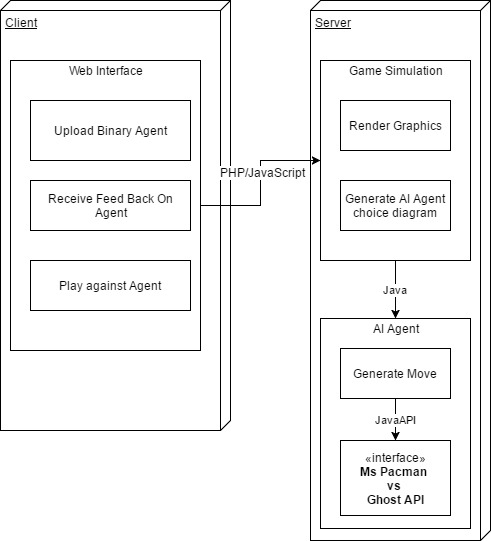
\includegraphics[width=8cm, height=8cm]{Images/RetroRabbit_Deployment_Diagram.jpg}\\[1cm]
\end{center}
       

\subsection{Development Methodology}

We will be utilizing \textbf{Agile} development methodologies with specific reference to \textbf{SCRUM} practices. We believe that this is the best means to enable both us as the engineering team and the client to focus on effectively performing the tasks integral to successfully providing the desired AI game playing agent. 
For this project, Retro Rabbit will take the part of \emph{Product Owner} and us as Panda Inc will be the \emph{Development Team}. Subsection 3 can be seen as rudimentary version of the \emph{Product Backlog} (which will be further refined/improved in the event of this tender being accepted).
\newline \newline
Interactions are highly valued by our team, hence we are dedicated to conducting weekly (at worst, bi-weekly) meetings with Retro Rabbit. As stated in the proposal, this will serve and start and end points for \emph{Sprints}. We will also be regularly meeting and consulting with our lectures and tutors for further guidance throughout the duration of the project. All of the above mentioned parties will have access a third party instant messaging platform in order to facilitate communication apart from physical meetings. Our team will be conducting bi-daily \emph{SCRUM meetings} in order to exchange our progress statuses and to ensure an comprehensive mutual understanding is maintained
\newline \newline
A collaborative and cooperative approach between both stakeholders will be employed for the life span of the project. There will also be a focus on the frequent, iterative presentation of small, incremental releases of deliverables to the client. The \textbf{role} of Retro Rabbit in this approach includes:
\begin{itemize}
\item Active involvement and collaboration in all phases of project
  \begin{itemize}
  \item Analysis and Design - The client will facilitate the identification, definition, prioritisation and continuous refinement of high level requirements, system architecture and design decisions of the AI game playing agent in order to ensure the correct functionality of the end product.
  \item Development and Deployment - The client will periodically review all instances of the product in order to ensure to it is in line with their expectations 
  \end{itemize}
\item Critical and constructive analysis on not only what we as the engineering team deliver but also on the quality of our service and whether or not we conducted ourselves as would be expected from those in a occupational environment
\item To provide us with the means to produce an effective end product. An exhaustive list of these required means will be provided in further Analysis and Design specification.
  
\end{itemize}

\begin{center}
{\fontfamily{UWR Grotesk}\sffamily\bfseries
\large Thank You RetroRabbit. We at Panda Inc. look forward to working with you in the near future.
}
\end{center}
\end{document}
